\documentclass[12pt]{article}
\usepackage{amsmath}
\usepackage{graphicx,psfrag,epsf}
\usepackage{enumerate}
\usepackage{natbib}
\usepackage{url} % not crucial - just used below for the URL 

%\pdfminorversion=4
% NOTE: To produce blinded version, replace "0" with "1" below.
\newcommand{\blind}{0}

% DON'T change margins - should be 1 inch all around.
\addtolength{\oddsidemargin}{-.5in}%
\addtolength{\evensidemargin}{-.5in}%
\addtolength{\textwidth}{1in}%
\addtolength{\textheight}{1.3in}%
\addtolength{\topmargin}{-.8in}%


%%%% Packages and definitions
\usepackage{amssymb}

\usepackage{xr}
\externaldocument{hillclimbing_jcgs_appendix}

\usepackage[top=0.85in,left=1.0in,right=1.0in,footskip=0.75in]{geometry}

% Use adjustwidth environment to exceed column width (see example table in text)
\usepackage{changepage}

% Use Unicode characters when possible
\usepackage[utf8]{inputenc}

% textcomp package and marvosym package for additional characters
\usepackage{textcomp,marvosym}

\usepackage[ruled]{algorithm}
\usepackage{algorithmic}

% cite package, to clean up citations in the main text. Do not remove.
\usepackage{cite}

% Use nameref to cite supporting information files (see Supporting Information section for more info)
\usepackage{nameref,hyperref}

%\usepackage{amsthm}

% ligatures disabled
\usepackage{microtype}
\DisableLigatures[f]{encoding = *, family = * }

% for the beautiful checkmarks
\usepackage{pifont}

\newtheorem{theorem}{Theorem}
\newtheorem{definition}{Definition}
\newtheorem{condition}{Condition}

\DeclareMathOperator*{\argmin}{arg\,min}


\begin{document}

%\bibliographystyle{natbib}

\def\spacingset#1{\renewcommand{\baselinestretch}%
{#1}\small\normalsize} \spacingset{1}


%%%%%%%%%%%%%%%%%%%%%%%%%%%%%%%%%%%%%%%%%%%%%%%%%%%%%%%%%%%%%%%%%%%%%%%%%%%%%%

\if0\blind
{
  \title{\bf Regularization Parameter Selection based on Validation-Error Descent with Non-smooth Criterions}
  \author{Jean Feng\thanks{
    Jean Feng was supported by NIH grants DP5OD019820 and T32CA206089.
    Noah Simon was supported by NIH grant DP5OD019820.
    The content is solely the responsibility of the authors and does not necessarily represent the official views of the National Institutes of Health.}\\
    Department of Biostatistics, University of Washington\\
    and \\
    Noah Simon \\
    Department of Biostatistics, University of Washington}
  \maketitle
} \fi

\if1\blind
{
  \bigskip
  \bigskip
  \bigskip
  \begin{center}
    {\LARGE\bf Regularization Parameter Selection based on Validation-Error Descent with Non-smooth Criterions}
\end{center}
  \medskip
} \fi

\bigskip
\begin{abstract}
In high-dimensional and/or non-parametric regression problems, regularization (or penalization) is used to control model complexity and induce desired structure. Each penalty has a weight parameter that indicates how strongly the structure corresponding to that penalty should be enforced. To tune these parameters, one common approach is to minimize the model error on a separate validation set. For problems with smooth optimization criterions, the gradient of the validation error with respect to the weights can be calculated. Hence a descent-based approach like gradient descent can be used. In this paper, we show how to calculate the exact gradient for problems with non-smooth penalty functions and provide an algorithm for tuning the parameters. The strength of this method is illustrated via simulations and a data analysis.
\end{abstract}

\noindent%
{\it Keywords:}  cross-validation, high-dimensional regression, regularization, optimization
\vfill

\newpage
\spacingset{1.45} % DON'T change the spacing!
\section{Introduction}
Consider the usual regression framework with $p$ features, $\boldsymbol x_i = (x_{i1},\ldots,x_{ip})^\top$, and a response $y_i$ measured on each of $i=1,\ldots,n$ observations. Let $\boldsymbol X$ denote the $n \times p$ design matrix and $\boldsymbol y$ the response vector. Our goal here is to characterize the conditional relationship between $\boldsymbol y$ and $\boldsymbol X$. In simple low-dimensional problems this is often done by constructing an $f$ in some pre-specified class $\mathcal{F}$ that minimizes a measure of discrepancy between $\boldsymbol y$ and $f(\boldsymbol X)$. Generally, this discrepancy is quantified with some pre-specified loss, $L$. Often $\mathcal{F}$ will endow $f$ with some simple form (e.g. a linear function). For ill-posed or high-dimensional problems ($p \gg n$), there can often be an infinite number of solutions that minimize the loss function $L$ but have high generalization error. A common solution is to use regularization, or penalization, to select models with desirable properties, such as smoothness and sparsity.

In recent years, there has been much interest in combining regularization methods to produce models with multiple desired characteristics. Examples include the elastic net \citep{zou2003regression}, which combines the lasso and ridge penalties, and the sparse group lasso \citep{simon2013sparse}, which combines the group lasso and lasso penalties. The general form of these regression problems is:
\begin{equation} \label {eq:basic}
\hat f(\boldsymbol{\lambda}) = \argmin_{f\in\mathcal{F}} L\left (\boldsymbol{y}, f (\boldsymbol{X}) \right ) + \sum\limits_{i=1}^J \lambda_i P_i(f)
\end{equation}
where $\{P_i\}_{i=1, ..., J}$ are the penalty functions and $\boldsymbol{\lambda} = (\lambda_1, \ldots, \lambda_J)^\top$ are the regularization parameters. 

Regularization parameters control the degree of various facets of model complexity, such as the amount of sparsity or smoothness. Often the goal is to set the parameters to minimize the fitted model's generalization error. One usually estimates this using a training/validation approach (or cross validation). There one fits a model on a training set $(\boldsymbol X_T, \boldsymbol y_T)$ and measures the model's error on a validation set $(\boldsymbol X_V, \boldsymbol y_V)$. The goal then is to choose penalty parameters $\boldsymbol{\lambda}$ that minimize the validation error, as formulated in the following optimization problem:
\begin{equation}
\begin{array}{c}
\min_{\boldsymbol{\lambda} \in \Lambda} L\left (\boldsymbol{y}_V, \hat f (\boldsymbol{X}_V | \boldsymbol{\lambda}) \right) \\
\text{s.t. } \hat f(\cdot | \boldsymbol{\lambda}) = \argmin_{f\in\mathcal{F}} L \left (\boldsymbol{y}_T, f (\boldsymbol{X}_T) \right) + \sum\limits_{i=1}^J \lambda_i P_i(f)
\end{array}
\label{jointopt}
\end{equation}
Here $\Lambda$ is some set that $\boldsymbol{\lambda}$ are known to be in, which is often just $\mathbb{R}^{J}_+$.

The simplest approach to solving \eqref{jointopt} is brute force: one fits models over a grid of parameter values and selects the model with the lowest validation error. As long as the grid is large and fine enough, this method of ``grid search" will find a solution close to the global optimum. Unfortunately, it is computationally intractable in cases with more than two parameters since the runtime is exponential in the number of parameters.

More efficient methods treat \eqref{jointopt} as a continuous optimization problem, generally through a gradient-free or gradient-based approach. Gradient-free approaches include the Nelder-Mead simplex algorithm \citep{nelder1965simplex} and Bayesian optimization \citep{snoek2012practical}, \citep{bergstra2011algorithms}, \citep{hutter2011sequential}. Although Bayesian optimization is currently the gold standard in machine learning, gradient-free methods are generally unable to tune more than twenty or so parameters whereas gradient-based methods can handle hundreds or even thousands of parameters. To calculate the gradient, one can use reverse-mode differentiation through the entire training procedure \citep{maclaurin2015gradient} or implicit differentiation of the KKT conditions \citep{larsen1998adaptive}, \citep{bengio2000gradient}, \citep{foo2008efficient}, \citep{lorbert2010descent}. To date, implicit differentiation methods have all required the optimization criterion to be smooth. In this paper, we show that the gradient can actually be calculated for many non-smooth regression problems, such as the lasso and the group lasso. Hence, we show that gradient descent, with some minor modifications, can be used to minimize the validation error over the penalty parameter space.

In Section~\ref{defineDescJointOpt}, we review descent-based optimization and give a gradient descent algorithm for minimizing the validation error over the penalty parameter space. Section~\ref{sec:results} presents three simulation studies comparing our method to gradient-free methods on regression problems with two to a hundred penalty parameters. We find that our method has superior performance in situations with twenty or more penalty parameters. Section~\ref{realDataResults} applies our method to gene expression data to predict colitis status.

% \eqref{jointopt} is generally not convex and thus we may not find the global minimum with a simple descent-based approach. However, in practice we find that simple descent gives competitive solutions.

\begin{bf}
Updates to the sections
\end{bf}
\begin{itemize}
\item{Section 2: remove ridge regression cause people might know it already? Add a discussion on the efficiency of the method for nonsmooth criterion. In the case of smooth criterions, the inverse of the Hessian is very expensive to calculate. For us, the inverse of the Hessian is cheap since the Hessian is extremely sparse.}
\item{Section 3: Have simulation studies with 2 - 5? penalty parameters comparing Bayesian Opt, Gradient Descent, Grid Search (if possible). We will need to discuss how Bayesian Opt is a bit weird to compare -- it doesn't require that many function evaluations, but requires time to update the Gaussian prior and also can't use warmstarts. Should we think about putting APLM with 3 penalties or Nonparametric additive model with 3 covariates?}
\item{Section 4: Have simulation studies with 20 - 100 penalty parameters? Should we just have the one group lasso example or should we add a second example? Perhaps we could have a nonparametric additive model with 30 covariates penalized by L1 trendfiltering or by sparsity-smoothness (basis function approach).}
\item{Section 6: We should add a discussion of the possibility of overfitting and how we want to do research on what happens when you add more parameters to tune via CV. Address the drawback that you really need to find a local minima for this method to work.}
\end{itemize}

\section{Descent-based Joint Optimization}\label{defineDescJointOpt}
\subsection{Definition}
In this manuscript we will restrict ourselves to classes $\mathcal{F} = \left\{f_{\boldsymbol \theta}\middle| \boldsymbol \theta\in\Theta\right\}$, which, for a fixed sample size $n$, are in some finite dimensional space $\Theta$. This is not a large restriction: the class of linear functions functions meets this requirement; as does any class of finite dimensional parametric functions. Even non-parametric methods generally either use a growing basis expansion (e.g. Polynomial regression, smoothing-splines, wavelet-based-regression, locally-adaptive regression splines \citep{tsybakov2008introduction}, \citep{wahba1981spline}, \citep{donoho1994ideal}, \citep{mammen1997locally}), or only evaluate the function at the observed data-points (eg. trend filtering, fused lasso, \citep{kim2009ell_1}, \citep{tibshirani2005sparsity}). In these non-parametric problems, for any fixed $n$, $\mathcal{F}$ is representable as a finite dimensional class.
We can therefore rewrite \eqref{eq:basic} in the following form:
\begin{equation}\label{eq:train_disc}
\argmin_{\boldsymbol \theta \in \Theta} L(\boldsymbol{y}, f_{\boldsymbol \theta}(\boldsymbol{X})) + \sum\limits_{i=1}^J \lambda_i P_i(\boldsymbol \theta)
\end{equation}

Suppose that we use a training/validation split to select penalty parameters $\boldsymbol{\lambda} = (\lambda_1, ..., \lambda_J)^\top$. Let the data be partitioned into a training set $(\boldsymbol{y}_T , \boldsymbol{X}_T)$ and validation set $(\boldsymbol{y}_V, \boldsymbol{X}_V)$. We can rewrite the joint optimization problem \eqref{jointopt} over this finite-dimensional class as:
\begin{equation}
\begin{array}{c}
\argmin_{\boldsymbol{\lambda} \in \Lambda} L(\boldsymbol{y}_V, f_{\hat{\boldsymbol \theta}(\boldsymbol{\lambda})}(\boldsymbol{X}_V)) \\
\text{s.t. } {\hat{\boldsymbol \theta}(\boldsymbol{\lambda})} = \argmin_{\boldsymbol \theta \in \Theta} L(\boldsymbol{y}_T, f_{\boldsymbol \theta} (\boldsymbol{X}_T)) + \sum\limits_{i=1}^J \lambda_i P_i(\boldsymbol \theta)
\end{array}
\label{jointopt2}
\end{equation}
For the remainder of the manuscript we will assume that \eqref{eq:train_disc} for the training set is strictly convex in $\boldsymbol \theta$. This ensures that there is a unique $\hat{\boldsymbol \theta}(\boldsymbol{\lambda})$ which perturbs continuously in $\boldsymbol{\lambda}$.

To ease exposition, we will assume throughout the remainder of the manuscript that $L \left( \boldsymbol{y}_V, f_{\boldsymbol \theta}(\boldsymbol{X}_V) \right)$ is differentiable in $\boldsymbol \theta$. This assumption is met if both 1) $f_{\boldsymbol \theta}(\boldsymbol{X}_V)$ is continuous as a function of $\boldsymbol \theta$; and 2) $L\left(\boldsymbol{y}_V,\cdot\right)$ is smooth. Examples include the squared-error, logistic, and poisson loss functions, though not the hinge loss.

\subsection{Smooth Training Criterion}
Here we present a brief summary of the approach of applying gradient descent when the training criterion is smooth. For more details, refer to \citet{bengio2000gradient}.

Let the training criterion be denoted as
\begin{equation}
L_T\left(\boldsymbol \theta, \boldsymbol{\lambda}\right) \equiv L(\boldsymbol{y}_T, f_{\boldsymbol \theta} (\boldsymbol{X}_T)) + \sum\limits_{i=1}^J \lambda_i P_i(\boldsymbol \theta)
\label{train}
\end{equation}
To calculate the gradient, we apply the chain rule
\begin{equation}
\nabla_{\boldsymbol{\lambda}} L \left( \boldsymbol{y}_V, f_{\hat{\boldsymbol \theta}(\boldsymbol{\lambda})}(\boldsymbol{X}_V) \right ) = 
\left [
\left . \frac{\partial}{\partial \boldsymbol \theta} L ( \boldsymbol{y}_V, f_{\boldsymbol \theta}(\boldsymbol{X}_V)) \right |_{\boldsymbol \theta=\hat{\boldsymbol \theta}(\boldsymbol \lambda)}
\right ]^\top 
\frac{\partial}{\partial \boldsymbol{\lambda}} \hat{\boldsymbol \theta}(\boldsymbol{\lambda})
\label{chainrule}
\end{equation}
The first term, $\frac{\partial}{\partial \boldsymbol \theta} L ( \boldsymbol{y}_V, f_{\boldsymbol \theta}(\boldsymbol{X}_V))$, is problem specific, but generally straightforward to calculate. To calculate the second term, $\frac{\partial}{\partial \boldsymbol{\lambda}} \hat{\boldsymbol \theta}(\boldsymbol{\lambda})$, we note that $\hat{\boldsymbol \theta}(\boldsymbol{\lambda})$ minimizes \eqref{train}. Since \eqref{train} is smooth,
\begin{equation}
\nabla_\theta 
L_T(\boldsymbol \theta, \boldsymbol{\lambda})
|_{\boldsymbol \theta = \hat {\boldsymbol \theta}(\boldsymbol{\lambda})}
= \boldsymbol{0}.
\label{eq:grad}
\end{equation}
Taking the derivative of both sides of \eqref{eq:grad} in $\boldsymbol{\lambda}$ and solving for $\frac{\partial}{\partial \boldsymbol{\lambda}} \hat{\boldsymbol \theta}(\boldsymbol{\lambda})$, we get:
\begin{equation}
\frac{\partial}{\partial \boldsymbol{\lambda}} \hat{\boldsymbol \theta}(\boldsymbol{\lambda}) = 
- \left . \left [
 \nabla_\theta^2 L_T (\boldsymbol \theta, \boldsymbol{\lambda} )^{-1}
\nabla_{\boldsymbol \theta} P(\boldsymbol \theta)
\right ]
\right |_{\boldsymbol \theta = \hat {\boldsymbol \theta}(\boldsymbol{\lambda})}
\label{implicitDifferentiation}
\end{equation}
where $\nabla_{\boldsymbol \theta} P(\boldsymbol \theta)$ is the matrix with columns $\{\nabla_{\boldsymbol \theta} P_i(\boldsymbol \theta)\}_{i=1:J}$.

We can plug \eqref{implicitDifferentiation} into \eqref{chainrule} to get $\nabla_{\boldsymbol{\lambda}} L \left ( \boldsymbol{y}_V, f_{\hat{\boldsymbol \theta}(\boldsymbol{\lambda})}(\boldsymbol{X}_V) \right )$. Note that because $\frac{\partial}{\partial \boldsymbol{\lambda}} \hat{\boldsymbol \theta}(\boldsymbol{\lambda})$ is defined in terms of $\hat{\boldsymbol \theta}\left(\boldsymbol{\lambda}\right)$, each gradient step requires minimizing the training criterion first. The gradient descent algorithm to solve \eqref{jointopt2} is given in Algorithm \ref{alg:smooth}.

\begin{algorithm}
\caption{Gradient Descent for Smooth Training Criterions}
\label{alg:smooth}
\begin{algorithmic}
        \STATE{
	        	Initialize $\boldsymbol{\lambda}^{(0)}$.
	}
        \FOR{each iteration $k=0,1,...$ until stopping criteria is reached}
        \STATE{
        		Solve for $\hat {\boldsymbol \theta}(\boldsymbol{\lambda}^{(k)}) = \argmin_{\boldsymbol \theta \in \Theta} L_T(\boldsymbol \theta, \boldsymbol{\lambda}^{(k)})$.
	}
        \STATE{
        		Calculate the derivative of the model parameters with respect to the regularization parameters
                        	\begin{equation}
                        \frac{\partial}{\partial \boldsymbol{\lambda}} \hat{\boldsymbol \theta}(\boldsymbol{\lambda}) = 
                        - \left . \left [ \left (
                         \nabla_\theta^2 L_T(\boldsymbol \theta, \boldsymbol{\lambda}^{(k)})  \right )^{-1}
                        \nabla_{\boldsymbol \theta} P(\boldsymbol \theta)
                        \right ]
                        \right |_{\boldsymbol \theta = \hat {\boldsymbol \theta}(\boldsymbol{\lambda}^{(k)})}
                        \label{eq:gradient_hessian}
                        	\end{equation}
	}
	\STATE{
		Calculate the gradient
                      \begin{equation}
                      \left .
                      \nabla_{\boldsymbol{\lambda}} 
                      L \left (\boldsymbol{y_V}, f_{\hat {\boldsymbol \theta}(\boldsymbol{\lambda})}(\boldsymbol{X_V}) \right)
                      \right |_{\boldsymbol{\lambda} = \boldsymbol{\lambda}^{(k)}} =
                      \left [ \frac{\partial}{\partial \boldsymbol \theta} L(\boldsymbol{y}_V, f_{\boldsymbol \theta}(\boldsymbol{X_V})) \Big |_{\theta = \hat \theta(\boldsymbol{\lambda}^{(k)})} \right ]^\top
                      \frac{\partial}{\partial \boldsymbol{\lambda}} \hat{\boldsymbol \theta}(\boldsymbol{\lambda}) \Big |_{\boldsymbol{\lambda}=\boldsymbol{\lambda}^{(k)}}
                      \end{equation}
        }
        \STATE{Perform gradient step with step size $t^{(k)}$
	\begin{equation}
	\boldsymbol{\lambda}^{(k+1)} := \boldsymbol{\lambda}^{(k)} -
	t^{(k)}
	\left . \nabla_{\boldsymbol{\lambda}} L \left( \boldsymbol{y}_V, f_{\hat{\theta}(\boldsymbol{\lambda})}(\boldsymbol{X}_V)  \right )
	\right |_{\boldsymbol{\lambda} = \boldsymbol{\lambda}^{(k)}}
	\end{equation}
	}
	\ENDFOR
\end{algorithmic}
\end{algorithm}



\subsection{Nonsmooth Training Criterion}
When the penalized training criterion in the joint optimization problem is not smooth, gradient descent cannot be applied. Nonetheless, we find that in many problems, the solution $\hat{\boldsymbol \theta}\left(\boldsymbol{\lambda}\right)$ is smooth at almost every $\boldsymbol{\lambda}$ (eg. Lasso, Group Lasso, Trend Filtering); this means that we can indeed apply gradient descent in practice. In this section, we characterize these problems that are almost everywhere smooth. In addition, we provide a solution for deriving $\frac{\partial}{\partial \boldsymbol{\lambda}} \hat{\boldsymbol \theta}(\boldsymbol{\lambda})$ since calculating the gradient is a challenge in and of itself. This is then incorporated into an algorithm for tuning $\boldsymbol{\lambda}$ using gradient descent.

To characterize problems that are almost everywhere smooth, we begin with three definitions:
\begin{definition}
The differentiable space of a real-valued function $L$ at a point $\boldsymbol \eta$ in its domain is the set of vectors along which the directional derivative of $L$ exists.
\begin{equation}
\Omega^{L}(\boldsymbol \eta) = \left \{ \boldsymbol u \middle | \lim_{\epsilon \rightarrow 0} \frac{L(\boldsymbol \eta + \epsilon \boldsymbol u) - L(\boldsymbol \eta)}{\epsilon} \text{ exists } \right \}
\end{equation}
\end{definition}

\begin{definition}
$S$ is a local optimality space for a convex function $L(\cdot, \boldsymbol \lambda_0)$ if there exists a neighborhood $W$ containing $\boldsymbol \lambda_0$ such that for every $\boldsymbol \lambda \in W$,
\begin{equation}
\argmin_{\boldsymbol \theta \in \Theta} L(\boldsymbol \theta, \boldsymbol \lambda) =
\argmin_{\boldsymbol \theta \in S} L(\boldsymbol \theta, \boldsymbol \lambda)
\end{equation}
\end{definition}

\begin{definition}
Let matrix $\boldsymbol B = [ \boldsymbol b_1 \hdots \boldsymbol b_p ] \in \mathbb{R}^{n \times p}$ have orthonormal columns. Let $f$ be a real-valued function over $\mathbb{R}^n$ and suppose its first and second directional derivatives of $f$ with respect to the columns in $\boldsymbol B$ exist. The Gradient vector and Hessian matrix of $f$ with respect to $\boldsymbol B$ are defined respectively as
\begin{equation}\label{eq:hess}
_{\boldsymbol B} \nabla f  =
\left (
\begin{array}{c}
\frac{\partial f}{\partial \boldsymbol b_1} \\
\frac{\partial f}{\partial \boldsymbol b_2} \\
\vdots\\
\frac{\partial f}{\partial \boldsymbol b_p}\\
\end{array}
\right ) \in \mathbb{R}^p;
\quad
_{\boldsymbol B}\nabla^2 f =
\left (
\begin{array}{cccc}
\frac{\partial^2 f}{\partial b_1^2} & \frac{\partial^2 f}{\partial b_1 \partial b_2} & ...  & \frac{\partial^2 f}{\partial b_1 \partial b_p} \\
\frac{\partial^2 f}{\partial b_2 \partial b_1} & \frac{\partial^2 f}{\partial b_2^2} & ...  & \frac{\partial^2 f}{\partial b_2 \partial b_p} \\
\vdots & \vdots &  \ddots & \vdots \\
\frac{\partial^2 f}{\partial b_p \partial b_1} & \frac{\partial^2 f}{\partial b_p \partial b_2} & ...  & \frac{\partial^2 f}{\partial b_p^2} \\
\end{array}
\right ) \in \mathbb{R}^{p \times p}
\end{equation}
\end{definition}

Using these definitions we can now give three conditions which together are sufficient for the differentiability of $L \left( \boldsymbol{y}_V, f_{\hat{\boldsymbol \theta}(\boldsymbol{\lambda})}(\boldsymbol{X}_V) \right )$ almost everywhere.

\begin{condition}
For almost every $\boldsymbol{\lambda}$, the differentiable space $\Omega^{L_T(\cdot, \boldsymbol{\lambda})}(\hat{\boldsymbol \theta}\left(\boldsymbol{\lambda}\right))$ is a local optimality space for $L_T\left(\cdot,\boldsymbol{\lambda}\right)$.
\end{condition}

\begin{condition}
For almost every $\boldsymbol{\lambda}$, $L_T\left(\cdot, \cdot\right)$ restricted to $\Omega^{L_T(\cdot, \cdot)}(\hat{\boldsymbol \theta}\left(\boldsymbol{\lambda}\right), \boldsymbol{\lambda})$ is twice continuously differentiable within some neighborhood of $\boldsymbol{\lambda}$.
\end{condition}

\begin{condition}
For almost every $\boldsymbol{\lambda}$, there exists an orthonormal basis $\boldsymbol B$ of $\Omega^{L_T(\cdot, \boldsymbol{\lambda})}(\hat{\boldsymbol \theta}\left(\boldsymbol{\lambda}\right))$ such that the Hessian of $L_T\left(\cdot, \boldsymbol{\lambda}\right)$ at $\hat{\boldsymbol \theta}\left(\boldsymbol{\lambda}\right)$ with respect to $\boldsymbol B$ is invertible.

\end{condition}
Note that if condition 3 is satisfied, the Hessian of $L_T \left(\cdot, \boldsymbol{\lambda}\right)$ with respect to any orthonormal basis of $\Omega^{L_T(\cdot, \boldsymbol{\lambda})}(\hat{\boldsymbol \theta}\left(\boldsymbol{\lambda}\right))$ is invertible.

Putting all these conditions together, the following theorem establishes that the gradient exists almost everywhere and provides a recipe for calculating it.

\begin{theorem}
Suppose our optimization problem is of the form in \eqref{jointopt2}, with $L_T\left(\boldsymbol \theta, \boldsymbol{\lambda}\right)$ defined as in \eqref{train}.

Suppose that $L \Big( \boldsymbol{y}_V, f_{\boldsymbol \theta}(\boldsymbol{X}_V)\Big)$ is continuously differentiable in $\boldsymbol \theta$, and conditions $1$, $2$, and $3$, defined above, hold.

Then the validation loss $L(\boldsymbol{y_V}, f_{\hat {\boldsymbol\theta}(\boldsymbol{\lambda})}(\boldsymbol{X_V}))$ is continuously differentiable with respect to $\boldsymbol{\lambda}$ for almost every $\boldsymbol{\lambda}$. Furthermore, the gradient of $L(\boldsymbol{y_V}, f_{\hat \theta(\boldsymbol{\lambda})}(\boldsymbol{X_V}))$, where it is defined, is
\begin{equation}
\nabla_{\boldsymbol{\lambda}} L \left ( \boldsymbol{y_V}, f_{\hat {\boldsymbol \theta}(\boldsymbol{\lambda})}(\boldsymbol{X_V}) \right) =
\left [ \left .
\frac{\partial}{\partial \boldsymbol \theta} L(\boldsymbol{y_V}, f_{\boldsymbol \theta}(\boldsymbol{X_V}))
\right |_{\boldsymbol \theta=\tilde{\boldsymbol \theta}(\boldsymbol \lambda)} \right ]^\top
\frac{\partial}{\partial \boldsymbol{\lambda}} \tilde{\boldsymbol \theta}(\boldsymbol{\lambda})
\end{equation}
where
\begin{equation}
\tilde{\boldsymbol \theta}(\boldsymbol{\lambda}) = \argmin_{\boldsymbol \theta \in \Omega^{L_T(\cdot, \boldsymbol{\lambda})}(\hat {\boldsymbol \theta}(\boldsymbol{\lambda}))} L_T(\boldsymbol \theta , \boldsymbol{\lambda})
\label{restrictedmodelparams}
\end{equation}
\label{thethrm}
\end{theorem}

We can therefore construct a gradient descent procedure based on the model parameter constraint in \eqref{restrictedmodelparams}. At each iteration, let matrix $\boldsymbol U$ have orthonormal columns spanning the differentiable space $\Omega^{L_T(\cdot, \boldsymbol{\lambda})}(\hat {\boldsymbol \theta}(\boldsymbol{\lambda}))$. Since this space is also a local optimality space, it is sufficient to minimize the training criterion over the column space of $\boldsymbol U$. The joint optimization problem can be reformulated using $\boldsymbol U \hat {\boldsymbol \beta}(\boldsymbol{\lambda})$ as the model parameters instead:
\begin{equation}
\begin{array}{c}
\min_{\boldsymbol \lambda \in \Lambda} L(\boldsymbol y_V, f_{\boldsymbol U \hat{\boldsymbol \beta} (\boldsymbol \lambda) }(\boldsymbol X_V)) \\
\text{s.t. } \hat{\boldsymbol \beta} (\boldsymbol \lambda) =
\argmin_{\boldsymbol \beta}
L_T (\boldsymbol U \boldsymbol \beta, \boldsymbol{\lambda} )
\end{array}
\end{equation}

This locally equivalent problem now reduces to the simple case where the training criterion is smooth. As mentioned previously, implicit differentiation on the gradient condition then gives us $\frac{\partial}{\partial \boldsymbol \lambda}\hat{\boldsymbol \beta}(\boldsymbol \lambda)$, which gives us the value of interest
\begin{equation}
\frac{\partial}{\partial \boldsymbol \lambda}
\hat{\boldsymbol \theta}(\boldsymbol \lambda) =
\boldsymbol U
\frac{\partial}{\partial \boldsymbol \lambda}\hat{\boldsymbol \beta}(\boldsymbol \lambda)
\end{equation}
Note that because the differentiable space is a local optimality space and is thus locally constant, we can treat $\boldsymbol U$ as a constant in the gradient derivations. Algorithm~\ref{alg:gradDescent} provides the exact steps for tuning the regularization parameters.

\begin{algorithm}
\caption{\label{alg:gradDescent} Joint Optimization with Gradient Descent}
  \begin{algorithmic}
        \STATE{
        		Initialize $\boldsymbol{\lambda}^{(0)}$.
	}
        \FOR { each iteration $k=0,1,...$ until stopping criteria is reached}
		\STATE{
              		Solve for $\hat {\boldsymbol \theta}(\boldsymbol{\lambda}^{(k)}) = \argmin_{\theta \in \Theta} L_T(\boldsymbol \theta, \boldsymbol{\lambda}^{(k)})$.
		}
              	\STATE{
			Construct matrix $\boldsymbol U^{(k)}$, an orthonormal basis of $\Omega^{L_T(\cdot, \boldsymbol{\lambda})}\left (\hat{\boldsymbol \theta}(\boldsymbol{\lambda}^{(k)}) \right )$.
		}
              	\STATE{
			Define the locally equivalent joint optimization problem
                            \begin{equation*}
                            \begin{array}{c}
                            \min_{\boldsymbol \lambda \in \Lambda} L(\boldsymbol y_V, f_{\boldsymbol U^{(k)} \hat{\boldsymbol \beta} (\boldsymbol \lambda) }(\boldsymbol X_V)) \\
                            \text{s.t. } \hat{\boldsymbol \beta} (\boldsymbol \lambda) =
                            \argmin_{\boldsymbol \beta}
                            L_T (\boldsymbol U^{(k)}\boldsymbol \beta, \boldsymbol{\lambda} )
                            \end{array}
                            \end{equation*}
		}              
              	\STATE{
			Calculate $\frac{\partial}{\partial \boldsymbol \lambda} \hat{\boldsymbol \beta}(\boldsymbol{\lambda})|_{\boldsymbol{\lambda} = \boldsymbol{\lambda}^{(k)}}$ where 
                               \begin{equation*}
                               \frac{\partial}{\partial \boldsymbol \lambda} \hat{\boldsymbol \beta}(\boldsymbol{\lambda}) =
                    		-  \left . \left[
				\left (
                    		_{\boldsymbol U^{(k)}}\nabla^2 L_T (\boldsymbol U^{(k)}\boldsymbol \beta, \boldsymbol{\lambda} )
                    		\right )^{-1}
                    		{}_{\boldsymbol U^{(k)}}\nabla P(\boldsymbol U^{(k)}\boldsymbol \beta)
				\right ]
                    		\right |_{\boldsymbol \beta =  \hat{\boldsymbol \beta}(\boldsymbol \lambda)}
                               \end{equation*}
			with $_{\boldsymbol U^{(k)}}\nabla^2$ and $_{\boldsymbol U^{(k)}}\nabla$ are as defined in \eqref{eq:hess}.
		}
              
              	\STATE{
			Calculate the gradient $\nabla_{\boldsymbol{\lambda}} L(\boldsymbol{y_V}, f_{\hat \theta(\boldsymbol{\lambda})}(\boldsymbol{X_V})) |_{\boldsymbol{\lambda} = \boldsymbol{\lambda}^{(k)}}$ where
                                 \begin{equation*}
                                 \nabla_{\boldsymbol{\lambda}} L \left (\boldsymbol{y_V}, f_{\hat \theta(\boldsymbol{\lambda})}(\boldsymbol{X_V}) \right ) =
                    		\left [
                    	  	\boldsymbol U^{(k)}
                    		\frac{\partial}{\partial \boldsymbol \lambda} \hat{\boldsymbol \beta}(\boldsymbol{\lambda})
                    		\right ]^\top
                    		\left [ \left .
                    		_{\boldsymbol U^{(k)}}\nabla L\left (\boldsymbol{y_V}, f_{\boldsymbol U^{(k)}\boldsymbol \beta}(\boldsymbol{X_V}) \right )
                                   	\right |_{\boldsymbol \beta = \hat{\boldsymbol \beta}(\boldsymbol \lambda)}
                    		\right ]
                                 \end{equation*}
		}
              \STATE{
              		Perform the gradient update with step size $t^{(k)}$
                            	\begin{equation*}
                            	\boldsymbol{\lambda}^{(k+1)} :=
                            	\boldsymbol{\lambda}^{(k)} - t^{(k)}
                            	\left .
                            	\nabla_{\boldsymbol{\lambda}} L \left (\boldsymbol{y_V}, f_{\hat \theta(\boldsymbol{\lambda})}(\boldsymbol{X_V}) \right )
                            	\right |_{\boldsymbol{\lambda} = \boldsymbol{\lambda}^{(k)}}
                            	\end{equation*}
		}
	\ENDFOR
  \end{algorithmic}
\end{algorithm}

Thus far we have restricted our attention to joint optimization for training/validation splits. Joint optimization for $K$-fold cross validation is described in the Appendix.

\subsection{Examples}\label{sec:examples}

To better understand the proposed gradient descent procedure, we present example joint optimization problems and their corresponding gradient calculations.

For ease of notation, we will let $S_{\boldsymbol{\lambda}}$ denote the differentiable space of $L_T(\cdot, \boldsymbol{\lambda})$ at $\hat{\boldsymbol{\theta}}(\boldsymbol{\lambda})$. All the example regressions satisfy the conditions in Theorem~\ref{thethrm}; details are included in the Appendix. Note that in some examples below, we add a ridge penalty with a fixed small coefficient $\epsilon > 0$ to ensure that the training criterion is strictly convex.

\subsubsection{Elastic Net}\label{sec:enet}

The elastic net \citep{zou2003regression}, a linear combination of the lasso and ridge penalties, is an example of a regularization method that is not smooth. We are interested in choosing regularization parameters $\boldsymbol{\lambda} = (\lambda_1, \lambda_2)^\top$ using the following joint optimization problem:
\begin{equation}
\begin{array}{c}
\min_{\boldsymbol{\lambda} \in \mathbb{R}^2_{+}} \frac{1}{2} \| \boldsymbol{y}_V - \boldsymbol{X}_V \hat{\boldsymbol{\theta}} (\boldsymbol \lambda) \| ^2 \\
\text{s.t. }
\hat{\boldsymbol{\theta}} (\boldsymbol{\lambda}) = \argmin_{\boldsymbol{\theta}} \frac{1}{2} \| \boldsymbol{y}_T - \boldsymbol{X}_T \boldsymbol{\theta} \| ^2
+ \lambda_1 \| \boldsymbol{\theta} \|_1
+ \frac{1}{2}\lambda_2 \| \boldsymbol{\theta} \|_2^2
\end{array}
\end{equation}

Let the nonzero indices of $\hat{\boldsymbol{\theta}}(\boldsymbol{\lambda})$ be denoted $I(\boldsymbol\lambda) = \{i | \hat{\theta}_i(\boldsymbol\lambda) \ne 0 \text{ for } i=1,...,p \}$ and let $\boldsymbol I_{I(\boldsymbol \lambda)}$ be a submatrix of the identity matrix with columns $I(\boldsymbol\lambda)$. Since $|\cdot|$ is not differentiable at zero, the directional derivatives of $||\boldsymbol \theta||_1$ only exist along directions spanned by the columns of $\boldsymbol I_{I(\boldsymbol \lambda)}$. That is, the differentiable space at $\boldsymbol \lambda$ is $S_{\boldsymbol{\lambda}} = span(\boldsymbol I_{I(\boldsymbol \lambda)})$.

Let $\boldsymbol{X}_{T, I(\boldsymbol\lambda)} = \boldsymbol{X}_T \boldsymbol{I}_{I(\boldsymbol \lambda)}$ and $\boldsymbol{X}_{V, I(\boldsymbol\lambda)}  = \boldsymbol{X}_V \boldsymbol{I}_{I(\boldsymbol \lambda)}$. The locally equivalent joint optimization problem is
\begin{equation}
\begin{array}{c}
\min_{\boldsymbol{\lambda} \in \mathbb{R}^2_{+}} \frac{1}{2} \| \boldsymbol{y}_V - \boldsymbol{X}_{V, I(\boldsymbol \lambda)} \hat{\boldsymbol{\beta}} (\boldsymbol \lambda) \| ^2 \\
\text{s.t. }
\hat{\boldsymbol{\beta}} (\boldsymbol{\lambda}) = \argmin_{\boldsymbol \beta} \frac{1}{2} \| \boldsymbol{y}_T - \boldsymbol{X}_{T, I(\boldsymbol \lambda)} \boldsymbol \beta \| ^2
+ \lambda_1 \| \boldsymbol \beta \|_1
+ \frac{1}{2}\lambda_2 \| \boldsymbol \beta \|_2^2
\end{array}
\end{equation}

To calculate the gradient, we can apply \eqref{implicitDifferentiation} since the training criterion is now smooth
\begin{equation}
\frac{\partial}{\partial \boldsymbol \lambda} \hat{\boldsymbol{\beta}}(\boldsymbol{\lambda}) = 
- \left ( 
\boldsymbol{X}_{T, I(\boldsymbol\lambda)}^\top \boldsymbol{X}_{T, I(\boldsymbol\lambda)} + \lambda_2 \boldsymbol{I}
\right )^{-1}
\begin{bmatrix}
sgn \left (\hat{\boldsymbol{\beta}} (\boldsymbol{\lambda}) \right ) &
\hat{\boldsymbol{\beta}} (\boldsymbol{\lambda})
\end{bmatrix}
\end{equation}
Hence, the gradient of the validation loss with respect to $\boldsymbol{\lambda}$ is
\begin{equation}
\nabla_{\boldsymbol \lambda} L(\boldsymbol{y_V}, f_{\hat{\boldsymbol{\theta}}(\lambda)}(\boldsymbol{X_V})) =
- \left (
\boldsymbol{X}_{V, I(\boldsymbol\lambda)}
\frac{\partial}{\partial \boldsymbol \lambda} \hat{\boldsymbol{\beta}}(\boldsymbol{\lambda})
\right )^{\top}
\left (
\boldsymbol y_V - \boldsymbol{X}_{V, I(\boldsymbol\lambda)} \hat{\boldsymbol{\beta}} (\boldsymbol{\lambda})
\right )
\end{equation}

\subsubsection{Additive Models with Sparsity and Smoothness Penalties}\label{sec:additive}

Now consider the nonparametric problem of modeling response $y$ given covariates $\boldsymbol{x} \in \mathbb{R}^p$. We suppose $y$ is the sum of $p$ univariate functions:
\begin{equation}
y = \sum_{i=1}^p f_i(x_i) + \epsilon
\end{equation}
Let $\boldsymbol{\theta}^{(i)} \equiv (f_i(x_{i1}), ..., f_i(x_{in}))$ be estimates of functions $f_i$ at the observations. As before, the model is fit using the least squares loss. In addition, we  encourage sparsity at the function level via group lasso penalties $\| \boldsymbol{\theta}_i \|_2$ and smoothness via lasso penalties on the second-order discrete derivatives of $f_i$. Below we will consider using a separate penalty parameter for each of the smoothness penalties, which can be particularly useful when some functions have nearly constant slope and other functions are very ``wiggly."

Define matrices $\boldsymbol{I}_T$ and $\boldsymbol{I}_V$ such that $\boldsymbol I_T \boldsymbol{\theta}^{(i)}$ and $\boldsymbol I_V \boldsymbol{\theta}^{(i)}$ are estimates for $f_i$ at the training and validation inputs, respectively. Let matrix $\boldsymbol{D}^{(2)}_{\boldsymbol{x}_i}$ be the second-order discrete difference operator input values $\boldsymbol{x}_i$. Construction of $\boldsymbol{D}^{(2)}_{\boldsymbol{x}_i}$ is given in the Appendix. Note that input values $\boldsymbol{x}_i$ from both the training and validation sets are incorporated into the matrices $\boldsymbol{D}^{(2)}_{\boldsymbol{x}_i}$ in order to estimate $f_i$ at all input points. The joint optimization problem is
\begin{equation}
\begin{array}{c}
\min_{\boldsymbol\lambda \in \mathbb{R}^{p+1}_{+}} \frac{1}{2|V|}
\left \|
\boldsymbol{y}_V
- \boldsymbol{I}_V \sum_{i=1}^p \hat{\boldsymbol{\theta}}^{(i)}(\boldsymbol{\lambda})
\right \|^2_2 \\
\text{s.t. }
\hat{\boldsymbol{\theta}}^{(i)}(\boldsymbol{\lambda}) =
\argmin_{\boldsymbol{\theta}}
\frac{1}{2} \left \|
\boldsymbol{y}_T
- \boldsymbol{I}_T \sum_{i=1}^p \boldsymbol{\theta}^{(i)} \right \|^2_2
+ \lambda_0 \sum_{i=1}^p \| \boldsymbol{\theta}^{(i)} \|_2 \\
+ \frac{1}{2} \sum_{i=1}^p \lambda_i \left \| \boldsymbol{D}^{(2)}_{\boldsymbol{x}_i} \boldsymbol{\theta}^{(i)} \right \|_1
+ \frac{1}{2} \epsilon \sum_{i=1}^p \| \boldsymbol{\theta}^{(i)} \|_2^2
\end{array}
\label{aplmProblem}
\end{equation}
Hence this training criterion contains $2p$ non-smooth penalty functions and $p+1$ penalty parameters.

The differentiable space is straightforward to determine for this problem, though requires bulky notation. Define $I_i(\lambda)$ for $i=1,...,p$ to be the indices along which smoothness penalty is not differentiable
\begin{equation}
I_i(\lambda) = \left \{j | \left (\boldsymbol{D}^{(2)}_{\boldsymbol{x}_i} \hat{\boldsymbol \theta}^{(i)}(\boldsymbol\lambda) \right )_j = 0 \text{ for } j=1,...,n \right \}
\end{equation}
and
\begin{equation}
J(\lambda) = \left \{ i | \hat{\boldsymbol \theta}^{(i)}(\boldsymbol\lambda) \ne \boldsymbol 0 \text{ for } i=1,...,p \right \}
\end{equation}
Also note that $\|\cdot\|_2$ is not differentiable in any direction at ${\bf 0}$ and is differentiable in all directions elsewhere. Then $S_{\boldsymbol \lambda} = span(\boldsymbol {U}^{(1)}) \oplus ... \oplus span(\boldsymbol {U}^{(p)}) $ where $\boldsymbol {U}^{(i)} = \boldsymbol{0}$ if $\hat{\boldsymbol \theta}^{(i)}(\boldsymbol\lambda) = \boldsymbol 0$ and $\boldsymbol {U}^{(i)}$ is an orthonormal basis of $\mathcal{N}(\boldsymbol{I}_{I_i(\lambda)}\boldsymbol{D}^{(2)}_{\boldsymbol{x}_i})$ otherwise.

Now we can define the locally equivalent joint optimization problem:
\begin{equation}
\begin{array}{c}
\min_{\boldsymbol{\lambda} \in \mathbb{R}^{p+1}_{+}}
\frac{1}{2|V|} \left \| \boldsymbol{y}_V
- \boldsymbol{I}_V \sum_{i\in J(\boldsymbol\lambda)} \boldsymbol {U}^{(i)} \hat{\boldsymbol{\beta}}^{(i)}(\boldsymbol{\lambda})
 \right \|^2_2 \\
\text{s.t. }
\hat{\boldsymbol{\beta}}^{(i)}(\boldsymbol{\lambda}) = \argmin_{\boldsymbol \beta}
\frac{1}{2n} \left \| \boldsymbol{y}_T
- \boldsymbol{I}_T \sum_{i\in J(\boldsymbol\lambda)} \boldsymbol {U}^{(i)} \hat{\boldsymbol{\beta}}^{(i)}(\boldsymbol{\lambda})
\right \|^2_2
+ \lambda_0 \sum_{i\in J(\boldsymbol\lambda)}  \| \boldsymbol {U}^{(i)} \boldsymbol{\beta}^{(i)} \|_2 \\
+ \frac{1}{2} \sum_{i\in J(\boldsymbol\lambda)} \lambda_i \left \| \boldsymbol{D}^{(2)}_{\boldsymbol{x}_i} \boldsymbol {U}^{(i)} \boldsymbol{\beta}^{(i)} \right \|_1
+ \frac{1}{2} \epsilon \sum_{i\in J(\boldsymbol\lambda)} \| \boldsymbol {U}^{(i)} \boldsymbol{\beta}^{(i)} \|_2^2
\end{array}
\end{equation}
From \eqref{implicitDifferentiation} and the chain rule, we get that the gradient of the validation loss is:
\begin{equation}
\nabla_{\boldsymbol \lambda} L(\boldsymbol{y_V}, f_{\hat{\boldsymbol{\theta}}(\boldsymbol{\lambda})}(\boldsymbol{X_V})) =
- \frac{1}{|V|}
\left (
\boldsymbol{I}_V \sum_{i\in J(\boldsymbol\lambda)}  \boldsymbol {U}^{(i)} \frac{\partial}{\partial \boldsymbol\lambda} \hat{\boldsymbol{\beta}}^{(i)}(\boldsymbol{\lambda})
\right )^\top
\left (
\boldsymbol{y}_V - \boldsymbol{I}_V \sum_{i\in J(\boldsymbol\lambda)} \boldsymbol {U}^{(i)} \hat{\boldsymbol{\beta}}^{(i)} (\boldsymbol\lambda)
\right )
\end{equation}
where
\begin{equation}
\frac{\partial}{\partial \lambda_i} 
\begin{bmatrix}
\hat{\boldsymbol{\beta}}^{1}(\boldsymbol{\lambda})\\
...\\
\hat{\boldsymbol{\beta}}^{|J(\boldsymbol{\lambda})|}(\boldsymbol{\lambda})\\
\end{bmatrix}
= \begin{cases}
\boldsymbol{H}(\boldsymbol\lambda)^{-1}
\begin{bmatrix}
\frac{\hat{\boldsymbol{\beta}}^{(1)}(\boldsymbol \lambda)}{||\boldsymbol {U}^{(1)}  \hat{\boldsymbol{\beta}}^{(1)} (\boldsymbol \lambda)||_2}\\
...\\
\frac{\hat{\boldsymbol \beta}^{(M)} (\boldsymbol \lambda)}{||\boldsymbol {U}^{(p)}  \hat{\boldsymbol{\beta}}^{(p)}(\boldsymbol \lambda)||_2}\\
\end{bmatrix}
& \text{ for } i = 0 
\\
\boldsymbol{H}(\boldsymbol\lambda)^{-1}
\begin{bmatrix}
\boldsymbol{0} \\
\boldsymbol {U}^{(i)\top}  \boldsymbol{D}^{(2)\top}_{\boldsymbol{x}_i} 
sgn( \boldsymbol{D}^{(2)}_{\boldsymbol{x}_i} \boldsymbol {U}^{(i)} \hat{\boldsymbol{\beta}}^{(i)}) \\
\boldsymbol{0} \\
\end{bmatrix}
& \text{ for } i \in J(\boldsymbol \lambda) \\
\boldsymbol{0}
& \text{ for } i \not\in J(\boldsymbol \lambda) \\
\\
\end{cases}
\end{equation}
The Hessian $\boldsymbol{H}(\boldsymbol\lambda)$ is defined in the Appendix.

%%% MOVE THIS MINI HESSIAN SECTION
Let 
\begin{equation}
\boldsymbol{U} = \begin{bmatrix}
\boldsymbol {U}^{(i_1)} & ... & \boldsymbol {U}^{(i_{|J(\boldsymbol \lambda)|})}
\end{bmatrix}
\end{equation}
where $i_\ell \in J(\boldsymbol \lambda)$. Then
\begin{equation}
\boldsymbol{H}(\boldsymbol\lambda)
= \boldsymbol{U}^\top \boldsymbol I_T^\top \boldsymbol I_T \boldsymbol{U}
+ \lambda_0 \text{ } diag \left (
\frac{1}{||\boldsymbol {U}^{(1)}  \hat{\boldsymbol{\beta}}^{(1)} (\boldsymbol \lambda)||_2} \left (
\boldsymbol I - \frac{\hat{\boldsymbol{\beta}}^{(1)} (\boldsymbol \lambda)^\top \hat{\boldsymbol{\beta}}^{(1)} (\boldsymbol \lambda)}{||\boldsymbol {U}^{(1)}  \hat{\boldsymbol{\beta}}^{(1)} (\boldsymbol \lambda)||_2}
\right ) \right )
+ \epsilon \boldsymbol I
\end{equation}

\subsubsection{Unpooled Sparse Group Lasso}\label{sec:sgl}

The sparse group lasso combines the $\|\cdot\|_2$ and $\|\cdot\|_1$ penalties, both of which are not smooth \citep{simon2013sparse}. This method is particularly well-suited for problems where features have a natural grouping, and only a few of the features from a few of the groups are thought to have an effect on response (e.g. genes in gene pathways). Here we consider a generalized version of sparse group lasso by considering individual penalty parameters for each group lasso penalty. This additional flexibility allows setting covariate and covariate group effects to zero by different thresholds. Hence un-pooled sparse group lasso may be better at modeling covariate groups with very different distributions.

The problem setup is as follows. Given $M$ covariate groups, suppose $\boldsymbol{X}$ and $\boldsymbol \theta$ are partitioned into $\boldsymbol{X}^{(m)}$ and $\boldsymbol \theta^{(m)}$ for groups $m = 1, ... , M$. We are interested in finding the optimal regularization parameters $\boldsymbol{\lambda} = (\lambda_1, \lambda_2)^\top$. The joint optimization problem is formulated as follows.
\begin{equation}
\begin{array}{c}
\min_{\boldsymbol{\lambda} \in \mathbb{R}^2_{+}} \frac{1}{2n}
\left \| \boldsymbol{y}_V - \boldsymbol{X}_V \hat{\boldsymbol{\theta}}(\boldsymbol{\lambda}) \right \|^2_2 \\
\text{s.t. }
\hat{\boldsymbol{\theta}}(\boldsymbol{\lambda}) =
\argmin_{\boldsymbol{\theta}} \frac{1}{2n} 
\left \| \boldsymbol{y}_T - \boldsymbol{X}_T \boldsymbol{\theta} \right \|^2_2
+ \lambda_0 \| \boldsymbol\theta \|_1
+ \sum_{m=1}^M  \lambda_m \| \boldsymbol\theta^{(m)} \|_2
+ \frac{1}{2} \epsilon \| \boldsymbol\theta \|_2^2
\end{array}
\label{eq:unpooled_sgl}
\end{equation}

Note the addition of a small, fixed ridge penalty to ensure strong convexity. As $\|\cdot\|_2$ (or $|\cdot|$) is not differentiable in any direction at ${\bf 0}$ (or $0$) and is differentiable in all directions elsewhere, it is straightforward to show that $S_{\boldsymbol \lambda} = span(\boldsymbol I_{I(\boldsymbol\lambda)})$ where $I(\boldsymbol\lambda) = \{i | \hat{\theta}_i(\boldsymbol\lambda) \ne 0 \text{ for } i=1,...,p \}$ are the nonzero indices of $\hat{\boldsymbol{\theta}}(\boldsymbol{\lambda})$.

To calculate the gradient, we define the locally equivalent joint optimization problem, using the same notational shorthand $\boldsymbol{X}_{T, I(\boldsymbol\lambda)}$ and $\boldsymbol{X}_{V, I(\boldsymbol\lambda)}$:
\begin{equation}
\begin{array}{c}
\min_{\boldsymbol{\lambda} \in \mathbb{R}^2_{+}} \frac{1}{2n} \left \| \boldsymbol{y}_V - \boldsymbol X_{V,I(\boldsymbol\lambda)} \hat{\boldsymbol\beta}(\boldsymbol{\lambda}) \right \|^2_2 \\
\text{s.t. }
\hat{\boldsymbol{\beta}}(\boldsymbol{\lambda}) = \argmin_{\boldsymbol \beta}
\frac{1}{2n} \left \| \boldsymbol{y}_T - \boldsymbol{X}_{T, I(\boldsymbol\lambda)} \boldsymbol \beta \right \|^2_2
+ \lambda_0 \| \boldsymbol \beta \|_1
+ \sum_{m=1}^M \lambda_m \| \boldsymbol \beta^{(m)} \|_2
+ \frac{1}{2}\epsilon \| \boldsymbol \beta \|_2^2
\end{array}
\end{equation}
From \eqref{implicitDifferentiation} and the chain rule, we get that the gradient of the validation loss is:
\begin{equation}
\nabla_{\boldsymbol \lambda} L(\boldsymbol{y_V}, f_{\hat{\boldsymbol{\theta}}(\boldsymbol{\lambda})}(\boldsymbol{X_V})) =
- \frac{1}{n}
\left (
\boldsymbol{X}_{V, I(\boldsymbol\lambda)}
\frac{\partial}{\partial \boldsymbol\lambda} \hat{\boldsymbol{\beta}}(\boldsymbol{\lambda})
\right )^\top
\left (
\boldsymbol{y}_V - \boldsymbol{X}_{V, I(\boldsymbol\lambda)} \hat{\boldsymbol{\beta}}(\boldsymbol{\lambda})
\right )
\end{equation}
where 
\begin{equation}
\frac{\partial}{\partial \boldsymbol \lambda} \hat{\boldsymbol{\beta}}(\boldsymbol{\lambda})
=
- \boldsymbol H(\boldsymbol \lambda)^{-1}
\begin{bmatrix}
\begin{bmatrix}
\frac{\hat{\boldsymbol{\beta}}^{(1)}(\boldsymbol \lambda)}{||\hat{\boldsymbol{\beta}}^{(1)} (\boldsymbol \lambda)||_2}\\
...\\
\frac{\hat{\boldsymbol \beta}^{(M)} (\boldsymbol \lambda)}{||\hat{\boldsymbol{\beta}}^{(M)}(\boldsymbol \lambda)||_2}\\
\end{bmatrix}
&
sgn(\hat{\boldsymbol{\beta}}(\boldsymbol{\lambda}))
\end{bmatrix}
\end{equation}
where the Hessian $\boldsymbol H(\boldsymbol \lambda)$ is given in the Appendix.

%% MOVE THE HESSIAN
\begin{equation}
\boldsymbol H(\boldsymbol \lambda) = \left (
\frac{1}{n} \boldsymbol{X}_{T, I(\boldsymbol\lambda)}^\top \boldsymbol{X}_{T, I(\boldsymbol\lambda)}
+ \boldsymbol{B}(\boldsymbol\lambda)
+ \epsilon \boldsymbol I_p
\right )
\end{equation}

\subsection{Gradient Descent Details}\label{sec:alg_details}
Here we discuss choice of step size and our convergence criterion.

There are many possible choices for our step size sequence $\{t^{(k)}\}$. Popular choices for convex problems are discussed in \citet{boyd2004convex}. We chose a backtracking line search as discussed in Chapter 9. In our examples initial step size was between 0.5 and 1 and we backtrack with parameters $\alpha \in [0.001, 0.01]$ and $\beta \in [0.01, 0.1]$. Details of backtracking line search are given in the Appendix. During gradient descent, it is possible that the step size will result in a negative regularization parameter; we reject any step that would set a regularization parameter to below a minimum threshold of $1e$-8.

Our convergence criterion is based on the change in our validation loss between iterates. More specifically, we stop our algorithm when
\[
L \left( \boldsymbol{y}_V, f_{\hat{\boldsymbol \theta}(\boldsymbol{\lambda}^{(k+1)})}(\boldsymbol{X}_V)\right) -
L \left( \boldsymbol{y}_V, f_{\hat{\boldsymbol \theta}(\boldsymbol{\lambda}^{(k)})}(\boldsymbol{X}_V)\right) \leq \delta
\]
for some prespecified tolerance $\delta$. For the results in this manuscript we use $\delta \in [1e\text{-}4, 1e\text{-}5]$.

\section{Simulation Studies}\label{sec:results}

We now compare our gradient descent algorithm to gradient-free methods through simulation studies. Each simulation corresponds to a joint optimization problem given in Section \ref{sec:examples}. We tune the regularization parameters over a training/validation split using gradient descent, Nelder-Mead, and the Bayesian optimization solver from \citet{snoek2012practical} called Spearmint. For baseline comparison, we also solve a two-parameter version of the joint optimization problem using grid search.

Inner training criterions were solved using the splitting conic solver (SCS) or ECOS in CVXPY \citep{cvxpy}, depending on the accuracy of the solver for the particular problem. Spearmint was allowed to solve the inner optimization problem at 100 penalty parameter points. Nelder-Mead was allowed fifty evaluations at each of the two initialization points. Grid search was performed over a $10 \times 10$ log-spaced grid. For comparison, we provide the number of times gradient descent solved the inner optimization problem (labeled ``\# Solves"). 

There are two potential computational concerns when tuning regularization parameters by gradient descent. First, the gradient calculation can be slow if the Hessian matrix in \eqref{eq:gradient_hessian} is large. \citet{bengio2000gradient} and \citet{foo2008efficient} suggest backpropagating through a Cholesky decomposition or using conjugate gradients (check this) to speed this up. This is actually not an issue for problems with non-smooth training criterions since the solutions tend to be sparse, which result in small Hessian matrices. The second concern is that the inner optimization problem must be solved to a high accuracy in order to calculate the gradient. (Recall that the gradient is derived via implicit differentiation.) To address this, we allow more iterations for solving the inner optimization problem. For a faster implementation of gradient descent, one can use a more specialized solver.

For each section below, we provide the simulation settings followed by a discussion of the results.

\subsection{Elastic Net}
Each dataset consists of 80 training and 20 validation observations with 250 predictors. The $\boldsymbol x_i$ were marginally distributed $N(\boldsymbol 0,\boldsymbol I)$ with $cor(x_{ij},x_{ik}) = 0.5^{|j-k|}$.
The response vector $\boldsymbol y$ was generated by
\begin{equation}
\boldsymbol y = \boldsymbol X \boldsymbol \beta + \sigma \boldsymbol \epsilon \; \text{where} \; \boldsymbol \beta = (\underbrace{1, ..., 1}_\text{size 15}, \underbrace{0, ..., 0}_\text{size 235})
\end{equation}
and $\boldsymbol \epsilon \sim N(\boldsymbol 0, \boldsymbol I)$. $\sigma$ was chosen such that the signal to noise ratio is 2. 

Grid search was performed over a $10 \times 10$ log-spaced grid from 1$e$-5 to 100. Nelder-mead and gradient descent were initialized at (0.01, 0.01) and (10, 10).

As shown in Table \ref{tab:elasticnet}, all the methods achieve similar validation errors. For this simple problem, the benefit for using gradient descent is not significant and gradient-free methods are simpler to implement.

\begin{table}
\caption {\label{tab:elasticnet} Comparison of solvers for Elastic Net joint optimization problem}
\centering
\begin{tabular}{| l | l | l | }
\hline
& Validation Error & \# Solves\\
\hline
% (1122 + 494 - 148 - 389)/30
Gradient Descent & 5.1963 (0.203) & 36.0 \\
\hline
Nelder-Mead & 5.1101 (0.196) & 50 \\
\hline
Spearmint & 5.4877 (0.219) & 100 \\
\hline
Grid Search & 5.2223 (0.1838) & 100 \\
\hline
\end{tabular}
\end{table}


\subsection{Additive model with Smoothness and Sparsity Penalty}
Each dataset consists of 150 training, 75 validation, and 75 test observations with $p=23$ covariates. The covariates $\boldsymbol{x_i} \in \mathbb{R}^{n}$ for $i=1,...p$ are equally spaced from -5 to 5 with a random displacement $ \delta \sim U(0, \frac{1}{300}) $ at the start and then shuffled randomly. The true model is the sum of three nonzero functions and 20 zero functions. Response $y$ was generated as follows
\begin{eqnarray*}
\boldsymbol y &=& \sum\limits_{i=1}^p \boldsymbol f_i(\boldsymbol x_i) + \sigma \boldsymbol \epsilon\\
f_1(x) &=& 9 \sin(3x)\\
f_2(x) &=& x\\
f_3(x) &=& 6 \cos(1.25 x) + 6 \sin(0.5 x + 0.5)\\
f_i(x) &=& 0 \text{ for }   i=4,...,23\\
\end{eqnarray*}
where $\boldsymbol \epsilon \sim N(\boldsymbol 0, \boldsymbol I)$. $\sigma$ was chosen such that the signal to noise ratio was 2.

Nelder-Mead and gradient descent were both initialized at $(10, 1, ..., 1)$ and $(0.1, 0.01, ..., 0.01)$. For baseline comparison, we also solved the two-parameter version of this joint optimization problem by pooling $\{\lambda_i\}_{i=1:p}$ into a single $\lambda_1$. Grid search then solved this problem by searching over a $10 \times 10$ log-spaced grid from 1$e$-4 to $100$. 

As shown in Table \ref{tab:additive}, the model from gradient descent over the joint optimization problem with $24$ penalty parameter achieved the lowest test error. Table \ref{tab:additive_average_lambda} provides the average penalty parameter values for $\lambda_0, ..., \lambda_4$. Gradient descent was indeed able to determine the smoothness of the functions. Among $f_1, f_2, f_3$, $f_1$ is the least smooth and $f_2$ is the most smooth. On average, gradient descent tuned $\lambda_1$ to have the smallest value and $\lambda_3$ to have the largest value. In contrast, Nelder-Mead wasn't able to determine the difference in smoothness between the functions and kept all penalty parameters the same. Spearmint chose a very different set of parameters that don't seem to be appropriate for the problem.

Figure \ref{fig:additive} provides an example model fitted by gradient descent for this joint optimization problem. As supported by Table \ref{tab:additive_average_lambda}, the fitted values $\boldsymbol {\theta}_1$ varies the most, followed by $\boldsymbol {\theta}_3$ and $\boldsymbol {\theta}_2$. Gradient descent also determined that $f_4$ was the zero function.

\begin{table}
\caption {\label{tab:additive} Additive model with $M+1$ penalty parameters vs. two penalty parameters. The parameters were tuned by gradient descent and grid search, respectively. Standard errors given in parentheses.}
\centering
\begin{tabular}{| l | l | l | l | l | }
\hline
& Num $\lambda$ & Validation Error & Test Error & \# Solves\\
\hline
% (729 + 351 - 87 - 184)/30
Gradient Descent & 24 & 23.9121 (0.930) & 26.1543 (0.781) & 27.0 \\
\hline
NM & 24 & 27.9132 (0.9044) & 28.7330 (0.897) & 100 \\
\hline
Spearmint & 24 & 32.6414 (2.033) & 37.7224 (2.173) & 100 \\
\hline
Grid Search & 2 & 28.8509 (0.916) & 30.0333 (0.9741) & 100 \\
\hline
\end{tabular}
\end{table}

\begin{table}
\caption {\label{tab:additive_average_lambda} Average $\lambda_i$ values for the fitted models}
\begin{tabular}{| l | l | l | l | l | l | }
\hline
& $\lambda_0$ & $\lambda_1$ & $\lambda_2$ & $\lambda_3$ & $\lambda_4$\\
\hline
Gradient Descent & 9.95813557 & 0.40320043 & 1.00567796 & 0.86451697 & 1.03670712 \\
\hline
Nelder-Mead & 9.68978106 & 0.90234764 & 1.00705168 & 0.99673684 & 1.00766817 \\
\hline
Spearmint & 3.3574752 & 0.76491086 & 0.0576163 & 0.00593712 & 0.03308817\\
\hline
Grid Search & 4.64731126 & 0.44005783 & -- & -- & -- \\
\hline
\end{tabular}
\end{table}

\begin{figure}
\centering
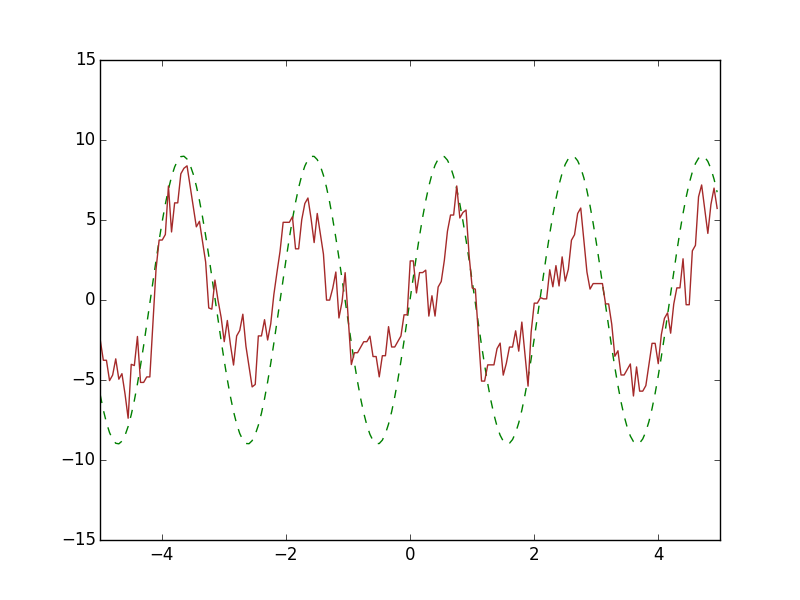
\includegraphics[height=50mm]{sparse_add_model_3_20_100_50_50_func0.png}
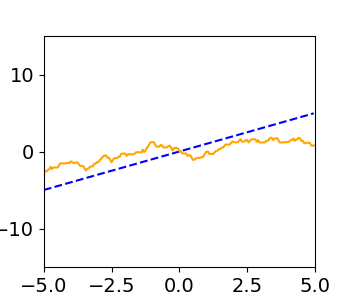
\includegraphics[height=50mm]{sparse_add_model_3_20_100_50_50_func1.png}
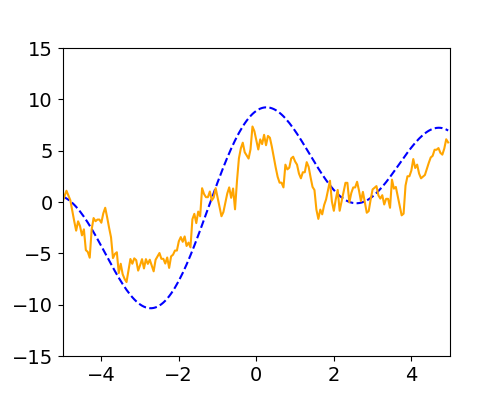
\includegraphics[height=50mm]{sparse_add_model_3_20_100_50_50_func2.png}
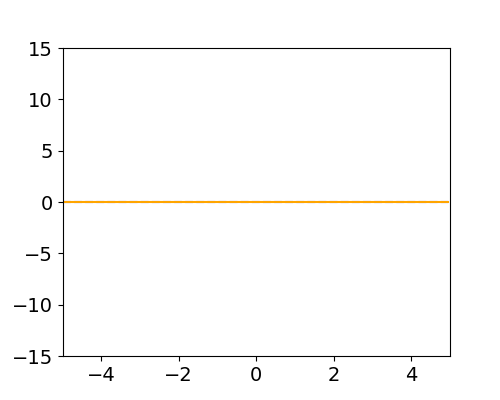
\includegraphics[height=50mm]{sparse_add_model_3_20_100_50_50_func3.png}
\caption{Example model fits given by gradient descent for $f_1, f_2, f_3,$ and $ f_4$. The dashed lines are the true functions and the solid lines are the estimated functions.}
\label{fig:additive}
\end{figure}


\subsection{Sparse group lasso}\label{sec:simulation_sgl}
We ran three experiments with different numbers of covariate groups $M$ and total covariates $p$, as given in Table \ref{table:unpooled}. For each experiment, the dataset consisted of $n$ training, $n/3$ validation, and 200 test observations. The predictors $\boldsymbol X$ were generated from a standard normal distribution. The response $\boldsymbol y$ was generated by
\begin{equation}
\boldsymbol y = \sum\limits_{j=1}^3 \boldsymbol X^{(j)} \boldsymbol \beta^{(j)} + \sigma \boldsymbol \epsilon \; \text{where} \; \boldsymbol \beta^{(j)} = (1, 2, 3, 4, 5, 0, ..., 0)
\end{equation}
where $\boldsymbol \epsilon \sim N(\boldsymbol 0, \boldsymbol I)$. $\sigma$ was chosen such that the signal to noise ratio was 2.

We compare joint optimization for the $M+1$ parameter problem to one with only two parameters, in which the $\{\lambda_i\}_{i=1:m}$ are pooled into a single $\lambda_2$. For the first experiment with 31 regularization parameters, we tune the parameters by gradient descent, Nelder-Mead, Spearmint, and Grid search (on the two-parameter version). The other two experiments had 61 and 101 regularization parameters and we compare the model from gradient descent to that from grid search on the two-parameter version. We didn't run Spearmint on the other two experiments since it is limited to problems with no more than forty hyperparameters. We also omit Nelder-Mead since it performed poorly and is not recommended for tuning so many parameters in general. For all problems, grid search was performed over a $10 \times 10$ grid from 1$e$-3 to $10$. Nelder-Mead and gradient descent were both initialized at $0.1 \times \boldsymbol 1$ and $\boldsymbol 1$.

Model performance was assessed using three metrics: test error, $\beta$ error (defined as $\| \boldsymbol \beta - \hat {\boldsymbol \beta} \|_2$), and the percentage of nonzero coefficients correctly identified among all the true nonzero coefficients. As shown in Table \ref{table:unpooled}, the model tuned by gradient descent produced the lowest test error and $\beta$ error in all three experiments. Interestingly, Nelder-Mead had the highest percentage of nonzero coefficients correctly identified in the first experiment. 

\begin{table}
\caption{\label{table:unpooled} Un-pooled sparse group lasso and sparse group lasso (SGL) tuned by gradient descent and grid search, respectively. Standard errors given in parentheses.}
\centering
\begin{tabular}{| l | l | l | l | l | l | }
\hline
\multicolumn{5}{|c|}{n=60, p=300, g=3, M=30}\\
\hline
 & $\beta$ Error & \% Correct Nonzero $\beta$ & Validation Error & Test Error & \# Solves \\
\hline
% 292 + 598 iters, 746 + 1518 CVX solves, (746 + 1518 - (292 + 598))/30 total solves
GD SGL & 7.2705 (0.303) & 17.3674 (0.934) & 22.5678 (1.720) & 47.5475 (2.995) & 45.8 \\
\hline
NM SGL & 8.4436 (0.2233) & 22.3932 (1.5002) & 57.2711 (4.0227) & 56.5659 (1.9765) & 100\\
\hline
SP SGL & 8.9100 (0.317) & 17.0926 (0.736) & 28.2522 (2.555) & 60.6027 (2.979) & 100\\
\hline
GS SGL & 8.4989 (0.250) & 15.9524 (1.186) & 52.3221 (3.664) & 56.8566 (2.097) & 100 \\
\hline
\multicolumn{5}{|c|}{n=90, p=900, g=3, M=60}\\
\hline
 & $\beta$ Error & \% Correct Nonzero $\beta$ & Validation Error & Test Error & \# Solves \\
\hline
% 578 + 344 iters, 1479 + 848 solves
GD SGL & 6.3492 (0.195) & 10.8078 (0.614) & 18.4029 (1.207) & 41.4825 (1.401) & 46.83 \\
\hline
GS SGL & 7.6669 (0.200) & 10.0291 (0.673) & 45.6976 (2.263) & 51.3434 (1.856) & 100 \\
\hline
\multicolumn{5}{|c|}{n=90, p=1200, g=3, M=100}\\
\hline
 & $\beta$ Error & \% Correct Nonzero $\beta$ & Validation Error & Test Error & \# Solves \\
\hline
%  iters 599 + 371, 1524 + 889 solves
GD SGL & 6.8224 (0.247) & 11.7190 (1.050) & 18.4298 (1.423) & 46.3634 (1.935) & 48.1 \\
\hline
GS SGL & 8.2767 (0.194) & 9.6516 (0.716) & 49.9974 (2.155) & 57.1398 (2.178) & 100 \\
\hline
\end{tabular}
\end{table}


\section{Application to Biological Data}\label{realDataResults}
Finally, we applied our algorithm in a real data example. More specifically, we considered the problem of finding predictive genes from gene pathways for Crohn's Disease and Ulcerative Colitis. \citet{simon2013sparse} addressed this problem using the sparse group lasso; we now compare this against applying the un-pooled sparse group lasso, where the regularization parameters were tuned using gradient descent. Since this is a classification task, the joint optimization problem is the same as \eqref{eq:unpooled_sgl} but with the logistic loss:
\begin{equation}
L\left ( \boldsymbol{y}, f_{\boldsymbol \beta(\boldsymbol\lambda)}(\boldsymbol{X}) \right ) = \sum_{i=1}^{n} y_{i} \log \left ( \frac{1}{1+\exp(-\boldsymbol x_{i}^\top \boldsymbol \beta)} \right ) + (1- y_i)\log \left (1 - \frac{1}{1+\exp(-\boldsymbol x_i^\top \boldsymbol \beta)} \right)
\end{equation}


Our dataset is from a colitis study of 127 total patients, 85 with colitis (59 crohn's patients + 26 ulcerative colitis patients) and 42 healthy controls \citep{burczynski2006molecular}. Expression data was measured for 22,283 genes on affymetrix U133A microarrays. We grouped the genes according to the 326 C1 positional gene sets from MSigDb v5.0 \citep{subramanian2005gene} and discarded the 2358 genes not found in the gene set.

We randomly shuffled the data and used the first 50 observations for the training set and the remaining 77 for the test set. Five-fold cross validation was used to fit models. To tune the penalty parameters in un-pooled sparse group lasso, we initialized gradient descent at $0.5 \times \boldsymbol 1$. For sparse group lasso, we tuned the penalty parameters over a $5 \times 5$ grid 1$e$-4 to 5.

Table \ref{colitis} presents the average results from repeating this process ten times. Un-pooled sparse group lasso achieved a slightly higher classification rate than sparse group lasso. Interestingly, un-pooled sparse group lasso found solutions that were significantly more sparse than sparse group lasso; on average, un-pooled sparse group lasso identified 9 genesets whereas sparse group lasso identified 38. These results suggest that un-pooling the penalty parameters in sparse group lasso could potentially improve interpretability.

In regards to runtime, we find that descent-based joint optimization for un-pooled sparse group lasso was computationally tractable, even though it required tuning 327 regularization parameters. In fact, it was slightly faster than grid-based joint optimization for sparse group lasso.

\begin{table}
\caption{\label{colitis} Predictive genes and genesets of Ulcerative Colitis found by un-pooled sparse group lasso vs. sparse group lasso (SGL). Standard errors given in parenthesis.}
\centering
\begin{tabular}{| l | l | l | l | l | }
\hline
 & \% Correct  & Num. Genesets & Num. Genes  \\
\hline
GD SGL & 88.57 (1.52) & 10.10 (0.995) & 51.80 (5.325) \\
\hline
GS SGL & 86.75 (1.7) & 30.8 (5.177) & 215.90 (20.841) \\
\hline
\end{tabular}
\end{table}

\section{Discussion}
In this paper, we proposed finding the optimal regularization parameters by treating it as an optimization problem over the regularization parameter space. We have proven that a descent-based approach can be used for regression problems in which the penalties are smooth almost everywhere and present a general algorithm for performing a modified gradient descent.

Empirically, we find that models fit by descent-based joint optimization have similar accuracy to those from grid search. Furthermore, the scalability of this approach allows us to test new regression problems with multiple penalties. In particular, we found that an un-pooled variant of sparse group lasso showed promising results. More research should be done to explore this new regularization method.

Future work could include finding other classes of regularization methods that are suitable for descent-based joint optimization and implementing descent-based joint optimization with more sophisticated optimization methods.

\bigskip

\bibliographystyle{agsm}
\bibliography{hillclimbing_nonsmooth}

\end{document}
